\documentclass[12pt]{scrartcl}

%\usepackage[utf8]{inputenc}
\usepackage[onehalfspacing]{setspace}
\usepackage[ngerman]{babel}
\usepackage{fontspec}
\usepackage[a4paper, left=3cm, right=3cm, top=3cm]{geometry}
\usepackage{amsmath}
%\usepackage{qtree}
\usepackage{listings}
\usepackage{floatrow}
%\usepackage{capt-of}
\usepackage{fancyvrb}
\usepackage{graphicx}
\usepackage[section]{placeins}
\usepackage{url}
\usepackage{multirow}
\usepackage{arydshln}

\floatstyle{plain}

\newfloat{program}{thp}{lop}
\floatname{program}{Beispiel}

\urldef\persalatin\url{http://www.perseus.tufts.edu/hopper/text?doc=Perseus%3atext%3a1999.04.0059}
\urldef\perselemlat\url{http://www.perseus.tufts.edu/hopper/text?doc=Perseus%3atext%3a1999.04.0060}
\urldef\vatlatinitas\url{http://www.vatican.va/roman_curia/institutions_connected/latinitas/documents/rc_latinitas_20040601_lexicon_it.html}
\lstdefinelanguage{gf}
{
  morekeywords={abstract, flags, cat, fun, incomplete, concrete, of, in, lincat, lin, resource, param, oper, variants, table, interface, instance, def, data, lindef, printname,},
  sensitive=false,
  morecomment=[l]{--},
  morestring=[b]",
  stringstyle={\textit}
}
\lstset{language=gf,captionpos=b,numbers=left, numberstyle=\tiny, numbersep=5pt}

\begin{document}
\setcounter{tocdepth}{3}
\date{30.9.2013}
\makeatletter

\begin{titlepage}
\begin{center}
\vspace{4cm}
\begin{huge}
Hausarbeit \\
zur Erlangung des Magistergrades \\
an der Ludwig-Maximilians-Universität München
\end{huge} \\[3cm]
{\Huge Erstellen einer Lateingrammatik im Grammatical Framework} \\[6cm]
{\LARGE vorgelegt von Herbert Lange} \\[5cm]
\end{center}
\parindent0mm
\begin{huge} 
Fach: Computerlinguistik  \\[0.3cm]
Referent: Prof. Dr. Klaus U. Schulz \\[0.3cm]
München, den \@date 
\end{huge}
\end{titlepage}
\makeatother
\tableofcontents
\pagebreak
\section{Einleitung}
\subsection{Motivation}
So mancher, der den Titel dieser Arbeit liest, wird sich wundern, warum man in der heutigen Zeit eine computergestützte Grammatik gerade für eine tote Sprache wie Latein entwickeln will. Doch die konkrete Sprache, die umgesetzt werden sollte, war bei der Wahl des Themas zunächst zweitrangig. Die Intention hinter dieser Arbeit war es eher, einmal in einem konkreten Falle die im Studium behandelten Theorien der Morphologie und der Syntax, aber auch die Prinzipien der Lexikonerstellung, in einem einheitlichen Projekt zusammenzuführen. \\
Das fuer dieses Unterfangen am ehesten geeignete Softwaresystem schien schon sehr bald das Grammatical Framework\footnote{\url{http://www.grammaticalframework.org/}} zu sein. Es stellt alle benötigten Hilfsmittel zur Verfügung, die jeweils für die einzelnen Komponenten benötigt werden, sorgt aber auch durch einen einheitlichen Beschreibungsformalismus für die nötige Konsistenz zwischen allen Bestandteilen. Weitere Vorteile des Grammatical Frameworks sind der mächtige Beschreibungsformalismus für Grammatiken, Unterstützung für Multilingualität und aktive Entwicklung als Open Source-Software. \\
Nachdem sich das Grammatical Framework als geeignet heraus gestellt hatte, fiel die Wahl der zu bearbeitenden Sprache auf Latein, da diese Sprache, die trotz ihres Alters in der Linguistik weiterhin nicht unbedeutend ist, in der Ressource Grammar Library\footnote{\url{http://www.grammaticalframework.org/lib/doc/synopsis.html}} bisher nur sehr rudimentär umgesetzt war. \\
\pagebreak
\subsection{Inhalt}
Im Folgenden sollen zunächst die Grundlagen der Arbeit genauer geschildert werden, es folgt also eine genauere Betrachtung des Grammatical Framework so wie der lateinischen Sprache. Anschließend wird das Vorgehen bei der Implementierung der Grammatik als zukünftiger Bestandteil der Ressource Grammar Library geschildert werden. Und zum Schluss soll noch eine Betrachtung der Erweiterungs- und Anwendungsmöglichkeiten folgen.
\pagebreak
\subsection{Das Grammatical Framework}
Das Grammatical Framework ist ein Softwaresystem mit einer spezialisierten Programmiersprache zur Entwicklung von Grammatiken. Es bietet alle nötigen Möglichkeiten um natürliche Sprachen zu verarbeiten. Dabei benutzt es Formalismen, wie sie auch in modernen funktionalen Programmiersprachen wie Haskell zu finden sind.\footnote{RANTA S. vii} Somit können einem manche Konzepte bereits vertraut sein, wenn man sich bereits mit den Möglichkeiten der funktionalen Programmierung auseinandergestzt hat.\\ 
Die große Stärke dabei ist die Multilingualität. Grundkonzept dabei ist die Trennung in eine konkrete und eine abstrakte Repräsentation der Grammatik. Dabei ist die abstrakte Struktur verschiedenen Sprachen gemein und die konkrete Syntax beschreibt, wie aus einem sprachunabhängigen Baum eine für die jeweilige Sprache spezifische Zeichenkette erzeugt werden kann. Über diesen Schritt der abstrakten Repräsentation kann man eine Übersetzung zwischen verschiedensten Sprachen umsetzen, die eine gemeinsame abstrakte Syntax teilen.\footnote{RANTA S. 10ff.} Dies Details dieses Formalismuses sollen nun genauer betrachtet werden.
\subsubsection{Der Grammatikformalismus}
Meist werden im Bereich der Computerlinguistik und Informatik kontextfreie Grammatiken, also Grammatiken von Typ 2 der Chomsky-Hierarchie verwendet.\footnote{quelle} Dies hat meist den Grund, dass die Mächtigkeit dieses Formalismuses meist ausreicht, die gewünschten Sprachen zu beschreiben, jedoch der Verarbeitungsaufwand vergleichsweise gering ist.\footnote{quelle}
\begin{program}[h]
\begin{tabular}{llll}
1 & S & $\longrightarrow$ & NP, VP \\
2 & NP & $\longrightarrow$ & Det, N \\
3 & N & $\longrightarrow$ & \textit{Mann} \\
4 & Det & $\longrightarrow$ & \textit{der} \\
5 & VP & $\longrightarrow$ & V \\
6 & V  & $\longrightarrow$ & \textit{schläft} \\
\end{tabular}
\caption{Kontextfreie Grammatikfragment}
\label{CFG-Beispiel}
\end{program}
Die in Beispiel \ref{CFG-Beispiel} gegebene Grammatik ist ein sehr minimalistisches Beispiel für eine kontextfreie Grammatik. Mit ihrer Hilfe kann nur der eine deutsche Satz \textit{Der Mann schläft} hergeleitet werden. Dabei hat eine mögliche Ableitung die in Beispiel \ref{CFG-Ableitung} gezeigte Form. Dabei wird top-down vorgegangen, also von der allgemeinsten Kategorie hinab bis zum spezifischen String. Alternativ wäre es auch möglich gewesen eine bottom-up-Ableitung anzugeben, die jedoch dem Ablesen der gegebenen Ableiung von unten nach oben entspricht. In der Grammatik sind die Regeln zum einfacheren Bezug auf die Grammatik mit Regelnummern versehen. Diese Regelnummern sind deshalb auch in der Ableitung und dem entsprechenden Syntaxbaum zu sehen.
\\
\begin{program}[h]
\begin{Verbatim}[commandchars=\\\{\},codes={\catcode`$=3\catcode`^=7}] 
S
$\overset{1}{\Rightarrow}$ NP VP
$\overset{2}{\Rightarrow}$ Det N VP
$\overset{4}{\Rightarrow}$ \textit{der} N VP
$\overset{3}{\Rightarrow}$ \textit{der Mann} VP
$\overset{5}{\Rightarrow}$ \textit{der Mann} V
$\overset{6}{\Rightarrow}$ \textit{der Mann schläft}
\end{Verbatim}
\caption{Ableitung des Satzes}
\label{CFG-Ableitung}
\end{program}
% $ Just to fix errors in syntax highlighting
\begin{figure}[h]
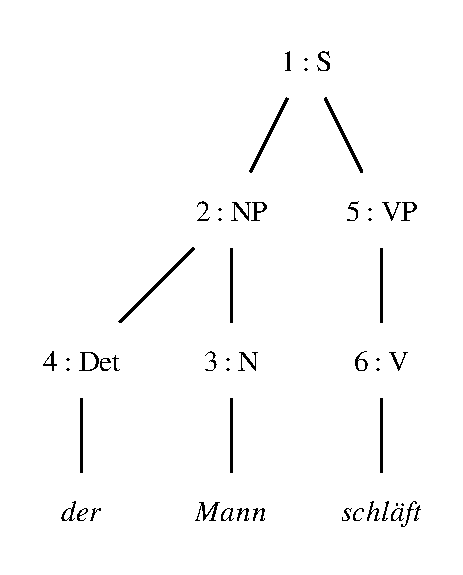
\includegraphics{minisatz/MiniSatzSyntax.eps}
\caption{Entsprechender Syntaxbaum}\label{CFG-Syntaxbaum}
\end{figure}
Im Formalismus des Grammatical Framework wird die oben gegebene Grammatik in die abstrakte und die konkrete Syntax zerlegt.
Dabei entspricht die abstrakte Syntax in etwa dem Syntaxbaum ohne die terminalen Blätter. Die abstrakte Syntax der kontextfreien Grammatik aus Beispiel \ref{CFG-Beispiel} ist in Listing \ref{GF-MiniSatzAbs} zu sehen. Zunächst gibt das Schlüsselwort \texttt{abstract} an, dass es sich um Datei mit einer abstrakten Syntaxbeschreibung handelt. Dieses Schlüsselwort wird vom Namen der Grammatik gefolgt. Anschließend folgt der Inhalt der Grammatik. \\
Zunächst werden mithilfe der \texttt{flags}-Direktive einige mögliche Einstellungen vorgenommen. In diesem sehr kurzen Beispiel wird nur die Startkategorie für das Parsing gesetzt, also die Wurzel aller Parsebäume. Andere mögliche Optionen sind z.B. die Einstellungen des Encodings und der Lexer, also das Programm, das die Eingabe in lexikalische Tokens zerlegt.\footnote{quelle} \\
Nach dem Schlüsselwort \texttt{cat} folgt eine Liste der nicht-lexikalischen Kategorien oder auch Nonterminal-Symbole. Sie entsprechen in etwa den Datentypen in (funktionalen) Programmiersprachen. \\
Hauptbestandteil der Grammatik sind offensichtlich die Syntaxregeln. Sie werden nach dem Schlüsselwort \texttt{fun} aufgelistet. Für denjenigen, der mit funktionaler Programmierung vertraut ist, kommt das Format der abstrakten Syntaxregeln möglicherweise bekannt vor, da es starke Ähnlichkeit zu Funktionensignaturen in Sprachen wie Standard ML oder Haskell hat. Dies ist allerdings kein Zufall, denn diese Regeln beschreiben lediglich die Bestandteile aus denen ein Ausdruck einer neuen Kategorie zusammengesetzt werden soll, ohne eine Aussage über das genaue Vorgehen zu treffen. Dies wird unabhänging voneinander in jeder konkreten Grammatik, die diese abstrakte Grammatik implementiert, beschrieben. So sagt die erste Regel mit dem Namen \texttt{mkNP} aus, dass ein Ausdruck der Kategorie \texttt{NP} aus einem Ausdruck der Kategorie \texttt{Det} und aus einem Ausdruck der Kategorie \texttt{N} zusammengesetzt werden kann. Die letzten drei Regeln führen lexikalische Einheiten mit einer entsprechenden Kategorie ein. \\
% Listing MiniSatzAbs
\lstinputlisting[float=ht,caption={Abstrakte Syntax},label={GF-MiniSatzAbs}]{minisatz/MiniSatzAbs.gf}
Diese abstrakte Grammatik kann nun konkret umgesetzt werden. Zwei konkrete Implementierungen, für Deutsch und Englisch, sind in Listing \ref{GF-MiniSatzGer} und \ref{GF-MiniSatzEng} zu finden. \\
% Listing MiniSatzGer
\lstinputlisting[float=ht,caption={Konkrete deutsche Syntax},label={GF-MiniSatzGer}]{minisatz/MiniSatzGer.gf}
% Listing MiniSatzEng
\lstinputlisting[float=ht,caption={Konkrete englische Syntax},label={GF-MiniSatzEng}]{minisatz/MiniSatzEng.gf}
Zunächst weist das Schlüsselwort \texttt{concrete} die Grammatik als eine konkrete Grammatik aus. Es folgt wie bei einer abstrakten Syntax der Name der Grammatik, diesmal wird jedoch darauf folgend angegeben welche abstrakte Grammatik die Grundlage bietet, hier unsere \texttt{MiniSatzAbs}-Grammatik. \\
Das in der deutschen, konkreten Grammatik verwendete Flag \texttt{coding} ermöglicht es, die Zeichenkodierung in den Zeichenketten festzulegen. In diesem Falle ist es für die deutschen Umlaute nötig das Encoding anzugeben.\footnote{quelle coding} Für andere Sprachen mit komplett vom lateinischen unterschiedlichen Schriftsystemen, gibt es auch die Möglichkeit statt der direkten Zeichenkodierung eine Transliteration zu verwenden.\footnote{quelle transliteration}\\
Das Schlüsselwort \texttt{lincat} ist die konkrete Entsprechung zum Schlüsselwort \texttt{cat} in der abstrakten Syntax. Hier müssen für jede in der abstrakten Syntax angegebene Kategorie ein konkreter Datentyp angegeben werden. In diesem Falle wurde für alle Kategorien der einfache Datentyp \texttt{Str}, also eine einfache Zeichenkette\footnote{Um genau zu sein, eine Liste von Tokens, die am Schluss mit Leerzeichen konkateniert werden}, gewählt. Das Grammatical Framework unterstützt auch verschiedene Arten komplexer Datentypen. \\
Auf den \texttt{lincat}-Block folgt, mit dem Schlüsselwort \texttt{lin} markiert, der Abschnitt, in dem die für jede abstrakte Syntaxregel beschrieben wird, wie diese in eine konkrete Zeichenkette zu übersetzen. Für die drei lexikalischen Regeln \texttt{Mann\_N}, \texttt{der\_Det} und \texttt{schlafen\_N} ist dies lediglich die entsprechende Zeichenkette z.B. für \texttt{Mann\_N} \textit{Mann} im Deutschen bzw. \textit{man} im Englischen. Die restlichen Syntaxregeln sind in diesem Beispiel nur geringfügig komplexer. Die Regel \texttt{mkVP} gibt lediglich den Parameter als Rückgabewert zurück, bildet also den gleichen String, der bereits als Parameter übergeben wurde. Und die beiden verbleibenden Regeln \texttt{mkNP} und \texttt{mkS} konkatenieren einfach die beiden als Parameter übergebenen Strings. \\
Man kann diese sehr kurzen konkreten Grammatiken zusammen mit der gemeinsamen Grammatik in das Grammatical Framework laden und in einer der beiden Sprachen den Satz \textit{der Mann schläft} bzw. \textit{the man sleeps} parsen und die abstrakte Representation \texttt{(mkS (mkNP der\_Det Mann\_N) (mkVP schlafen\_V))} in die andere Sprache linearisieren, also mit Hilfe der konkreten Syntaxregeln die entsprechende Zeichenkette in der Sprache generieren. \\
\begin{figure}
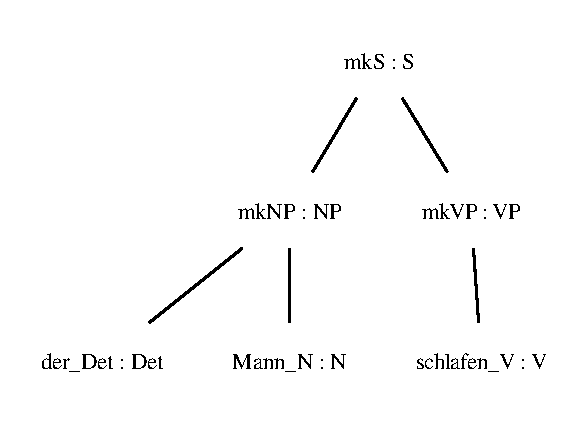
\includegraphics{minisatz/MiniSatzTree.eps}
\caption{Baum der abstrakten Syntax}\label{MiniSatz-AbsTree}
\end{figure}
\begin{figure}
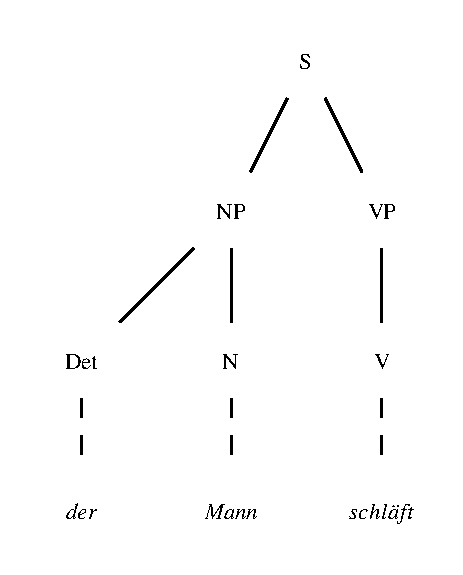
\includegraphics{minisatz/MiniSatzParseGer.eps}
\caption{Parsebaum der konkreten deutschen Syntax}\label{MiniSatz-ParseGer}
\end{figure}
Mit Hilfe des Grammatical Frameworks kann man auch verschiedene Bäume beim Parsen grafisch darstellen lassen. Zum einen den abstrakten Syntaxbaum und zum anderen den konkreten Parsebaum für eine der implementierten Sprachen. Diese Bäume für die MiniSatz-Grammatik sind in Abb. \ref{MiniSatz-AbsTree} und \ref{MiniSatz-Parse-Ger} zu sehen.
% Listing SatzAbs
\lstinputlisting[float=ht,caption={Erweiterte abstrakte Syntax},label={GF-SatzAbs}]{satz/SatzAbs.gf}
Nun kann man diese doch sehr minimalistische Grammatik etwas erweitern, so dass man auch die Sätze ``die Frauen schlafen'', ``der Mann sieht die Frau'' und ``der Mann liest das Buch''erkennen kann. Die fertigen Quelltextdateien sind in Listing \ref{GF-SatzAbs}, \ref{GF-SatzGer} und \ref{GF-SatzEng} zu finden. Die Veränderungen in der abstrakten Syntax (Listing \ref{GF-SatzAbs} sind nicht sehr umfangreich und betreffen hauptsächlich die Einführung von transitiven Verben mit der Kategorie \texttt{V2}. Mit der Funktion \texttt{mkVP2} wird aus einem transitiven Verb und einer Nominalphrase eine Verbalphrase mit Akkusativobjekt aufgebaut. Um auch Nominalphrasen im Plural zu ermöglichen, wird für den bestimmten Artikel eine Singular- und eine Pluralform benötigt. Sonst wird noch das ``Lexikon'' um die Wörter für Frau, Buch, sehen und lesen erweitert. \\
% Listing SatzGer
\lstinputlisting[float=ht,caption={Erweiterte konkrete deutsche Syntax},label={GF-SatzGer}]{satz/SatzGer.gf}
In der konkreten Umsetzung sind nun aber größere Unterschiede, sowohl zur ursprünglichen Grammatik, als auch zwischen den unterschiedlichen Sprachen zu finden. [fehlt: Beschreibung der konkreten Programme]
% Listing SatzEng
\lstinputlisting[float=ht,caption={Erweiterte konkrete englische Syntax},label={GF-SatzEng}]{satz/SatzEng.gf}
\FloatBarrier
\subsubsection{Die Ressource Grammar Library}
Was für allgemeine Programmiersprachen eine Standardbibliothek ist, ist im Grammatical Framework für die Multilingualität die Ressource Grammar Library. Sie ist definiert als gemeinsame abstrakte Syntax, die für verschiedenen Sprachen implementiert ist. Auf diese Möglichkeit ist eine grundlegende Übersetzung zwischen den unterstützten Sprachen direkt nach der Installation möglich. Meist muss jedoch mindestens das nötige Vokabular angegeben werden, da das Lexikon auf eine kleine Anzahl von Wörtern beschränkt ist, die benötigt wird um die grammatischen Konstrukte zu testen. \\
% Listing RglSatzAbs
\lstinputlisting[float=ht,caption={Abstrakte Syntax mit Hilfe der RGL},label={GF-RglSatzAbs}]{rglsatz/RglSatzAbs.gf}
% Listing RglSatzGer
\lstinputlisting[float=ht,caption={Konkrete deutsche Syntax mit Hilfe der RGL},label={GF-RglSatzGer}]{rglsatz/RglSatzGer.gf}
% Listing RglSatzEng
\lstinputlisting[float=ht,caption={Konkrete englische Syntax mit Hilfe der RGL},label={GF-RglSatzEng}]{rglsatz/RglSatzEng.gf}
\pagebreak
\FloatBarrier
\subsection{Die Lateinische Sprache}
\subsubsection{Sprachwissenschaftliche Einordnung}
Die lateinische Sprache, auch als oskisch-umbrische Sprache bezeichnet, gehört zur indogermanische Sprachfamilie und dort zur Unterfamilie der italischen Sprachen. Durch diese Verwandschaft kann man bei Wörtern und Wortformen oft Entsprechungen zwischen der lateinischen Sprache und verschiedensten anderen Sprachen Westeuropas bis hin zu Mittelasien finden (vgl. Tabelle \ref{Idg-Entsprechungen}.\footnote{vgl. BAYER-LINDAUER1994 S.1}
\begin{table}[h]
\begin{tabular}{|l|l|l|}
\hline
lateinisch & altgriechisch & deutsch \\
\hline
pater & \pi\alpha\tau\'{\eta}\rho\ (=patēr) & Vater \\
ager & \alpha\gamma\rho\'{o}\varsigma\ (=agr\'{o}s)& Acker \\
trēs & \tau\rho\varepsilon\~{\iota}\varsigma\ (=treĩs) & drei \\
decem & \delta\'{\varepsilon}\kappa\alpha\ (=d\'{e}ka) & zehn \\
\hline
\end{tabular}
\caption{Wortentsprechungen in verschiedenen indogermanischen Sprachen (vgl. BAYER-LINDAUER S.1)}
\label{Idg-Entsprechungen}
\end{table}
Entstanden ist es als ein in der Stadt Rom üblicher Dialekt parallel zu anderen ländlicheren Dialekten im Latium, im laufe der Zeit verdrängte es jedoch die weiteren italischen Sprachen im Zuge der Ausdehnung des römischen Reichs.\footnote{vgl. METZLER2004 S. 5359} Die Sprachgeschichte kann in mehrere Epochen unterteilt werden. Üblicherweise beginnt man diese Einordnung mit der Epoche des Altlateins, das von ca. 240 v. Chr bis 80 v. Chr angesiedelt wird. Es reicht von den frühesten nachgewiesenen lateinischen Sprachzeugnissen bis zum Beginn der Zeit des klassischen Lateins. Dessen Zeitaum wird von ca. 80 v. Chr. bis 117. n. Chr. gerechnet und beginnt in etwa mit den ersten öffentlichen Auftritten des M. Tullius Cicero. Die bekannten Gerichtsreden des berühmten römischen Anwalts und Schriftstellers von ca. 80 v. Chr sind noch größtenteils erhalten. Die nachklassische Phase kann wiederum in verschiedene Epochen unterteilt werden, in denen unter anderem die romanischen Volkssprachen entstanden sind, bis hin zum sogenannten Neulatein, das noch vom 15. Jahrhundert bis hin zum beginn des 20. Jahrhundert die Sprache der Wissenschaft darstellte und auch heute noch großen Einfluss auf Begriffe des Alltags ausübt.\footnote{MÜLLER-LANCE2006 S. 27ff.}  \\
Auch heute noch am bedeutendsten ist jedoch wohl das klassische Latein, das weiterhin in Schulen unterrichtet wird und sich vor allem mit seinem großen überlieferten Textkorpus hervorhebt. Da sich die meisten Lateingrammatiken auf diese Sprachepoche stützen, wird diese primär in dieser Arbeit betrachtet.\footnote{quelle}. \\
In der Sprachwissenschaft ist jedoch auch weiterhin umstritten, in welchem Verhältnis das klassische Latein zum sogenanten Vulgärlatein steht. Heutzutage geht man davon aus, dass das klasische Latein eine kaum wirklich gesprochene Sprache war und das Vulgärlatein nicht nur eine nachklassische Sprachvariante ist, sondern bereits parallel zum klasischen Schriftlatein als gesprochene Sprache verwendet wurde. Allerdings fand das klassische Latein noch bis in das 5. Jahrhundert n. Chr. Verwendung als eine Art Schreibnorm, während sich das Vulgärlatein langsam hin zu den romanischen Sprachen entwickelte.\footnote{vgl. METZLER2004 S. 5359 und S. 10719} \\
Formal gehört Latein den stark flektierenden Sprachen. Das heißt das in der lateinischen Sprache, wie für synthetische Sprachen üblich, syntaktische Klassen und Verhältnisse über Wortsuffixe ausgedrückt werden.\footnote{vgl. METZLER2004 S. 9690}. Allerdings drücken bei flektierenden Sprachen, im Gegensatz zu agglutinierenden Sprachen, die Affixe meist mehr als en grammatisches Merkmal aus.\footnote{vgl. METZLER2004 S. 3009} So ist bei der Verbform \textit{audio} das \textit{audi} der Verbstamm, um genau zu sein den Präsensstamm, des Verbs \textit{audire} und das Suffix \textit{-o} kodiert folgende Merkmale: 1. Person, Singular, Präsens, Indikativ, Aktiv.\footnote{vgl. BAYER-LINDAUER1994 S. 75} \\
Es gibt fünf zum Teil genusbasierte Flexionsklassen\footnote{Def. Flexionsklasse} für Nomen, sechs verschiedene Kasus (Nominativ, Genitiv, Dativ, Akkusativ, Ablativ und Vokativ), drei Genera (Maskulin, Feminin, Neutrum), ein voll flektierendes Pronomensystem und vier relativ stark synthetische Flexionsklassen für Verben.\footnote{METZLER2004 S. 5359} Zu den Kasus sei anzumerken, dass der Ablativ im Lateinischen ein eigenständiger Kasus ist, jedoch der Vokativ oft mit dem Nominativ zusammenfällt.\footnote{vgl. BAYER-LINDAUER1994 S. 20f.} \\
Die Wortstellung des Lateinischen wird oft als sehr frei beschrieben, allerdings gibt es eine klare Präferenz der SOV-Wortstellung im Satz, also dass das Objekt des Satzes direkt auf das Subjekt folgt, und das Verb den Satz abschließt. Die Möglichkeiten zur Positionierung des Adjektivs im Bezug auf das Nomen sind allerdings durch nichts beschränkt.\footnote{METZLER2004 s. 5359}
\subsubsection{Bedeutung in der heutigen Zeit}
Man kann sich natürlich über die Notwendigkeit streiten, sich in der heutigen Zeit noch mit der lateinischen Sprache zu beschäftigen. Es gibt aber auch ziemlich gute Gründe dafür Latein nicht einfach nur als tote Sprache abzustempeln und nicht weiter zu betrachten. \\
Der am häufigsten, vor allem im Schulalter bei der Wahl einer zu lernenden Fremdsprache, vorgebrachte Grund ist, dass die lateinische Sprache als ``Mutter aller romanischen Sprachen'' später einen einfacheren Einstieg in das Erlernen z.B von Französisch oder Spanisch bietet. Auch gilt Latein galt seit Jahrhunderten, und gilt weiterhin, als produktive Quelle für Fachbegriffe aus Wissenschaft, Forschung und Technik. So haben viele moderne Begriffe wie Computer\footnote{von \textit{lat.} computere - berechnen} und Monitor\footnote{\textit{lat.} f. der Mahner, von \textit{lat.} monere - mahnen} lateinische Wurzeln. Auch im Universitätsalltat wird man oft mit lateinischen Lehnwörtern konfrontiert. Man trifft sich zum Essen in der Mensa\footnote{\textit{lat.} mensa - Tisch, Tafel} und studiert an Fakultäten\footnote{von \textit{lat.} facultas - Vermögen, Fähigkeit}. \\
Vor allem in der Sprachwissenschaft hat Latein eine besondere Bedeutung, da sie bei einem Vergleich verschiedener indogermanischer Sprachen als eine Art \textit{default}-Sprache angesehen werden kann, denn sie bietet fast alle nötigen grammatischen Kategorien, die gewöhnlich benötigt werden. So kann Latein als Vergleichsparameter (\textit{tertium comparationis}) verwendet werden. Diese Stellung der lateinischen Sprache spiegelt sich auch in der Fachterminologie moderner Schulgrammatiken wieder, die fast ausschließlich von lateinischen Fachausdrücken geprägt ist.\footnote{vgl. MÜLLER-LANCE2006 S. 10} \\
Als etwas skurile Verwendung einer Variation der lateinischen Sprache kann \textit{latino sine flexione} gelten. Diese von Giuseppe Peano anfang des 20. Jahrhunderts als Welthilfssprache entwickelte vereinfachte Form der lateinischen Sprache fand bis ca. 1950 in mehreren wissenschaftlichen Veröffentlichungen Verwendung. Sie basiert auf dem üblichen lateinischen Wortsschatz, der auch durch modernes romanisches Vokabular erweitert werden kann, und einer stark vereinfachten Morphologie.\footnote{vgl. METZLER2004 S. 5374}
\pagebreak
\section{Grammatikerstellung}
Nach der Einführung in die nötigen Grundlagen, um die Schritte zu verstehen, die nötig sind um im Grammatical Framework eine Grammatik zu entwickeln, folgt nun eine Schilderung der konkreten Schritte die nötig waren um eine Lateingrammatik im Grammatical Framework zu entwickeln. \\
Es sei noch anzumerken, dass es bereits früher Bestrebungen von Aarne Ranta gab, eine Lateingrammatik für die Ressource Grammar Library des Grammatical Frameworks zu entwickeln. Diese Arbeit baut auf diesen ersten Versuchen auf, kann aber insofern als selbständige und vollwertige Arbeit angsehen werden, da die bisherige implementierung sehr rudimentär war und seit ca. 2005 nicht mehr weiterentwickelt wurde. Im Anhang C ist der Quelltext meiner Arbeit als sogenanntes Diff\footnote{} zum Zustand vor Beginn der Arbeit zu finden. \\
Die Gliedering folgt dem gewählten Vorgehen bei der Implementierung. Die Begründung für die Reihenfolge der einzelnen Schritte wird jeweils zu Beginn der einzelnen Kapitel kurz dargelegt.
\pagebreak
\subsection{Lexikon}
Den Beginn dieser Grammatikimplementierung bildete die Erstellung des minimal nötigen Lexikons. Durch die abstrakte Syntax der RGL\footnote{vgl. \textbf{lib/src/abstract/Lexicon.gf} und \textbf{lib/src/abstract/Structural.gf}} ist eine Liste von etwas über 450 englischen Bezeichnern für Worte vorgegeben, die in jeder Sprache umgesetzt werden sollten. \\
Für die Erstellung eines Lexikon, wie es in einer Grammatik verwendet werden kann, sind zwei Schritte nötig. Einerseits müssen für jeden vorgegebenen Bezeichner, in diesem Falle alle lexikalischen Funktionen aus dem abstrakten Lexikon die zugeordneten Zeichenketten zugeordnet werden. Und zum anderen muss das Lexikon auch all jene Informationen enthalten, die später zum bilden der Vollformen und zur Konstruktion grammatischer Einheiten nötig sind.
Der erste Schritt dabei begann damit, einfach das Lexikon einer anderen Sprache, in diesem Falle Englisch, zu kopieren. Normalerweise ist es vernünftiger, mit einer Sprache zu beginnen, die der zu implementierenden Sprache möglichst nahe steht.\footnote{RGL beginn}. Allerdings wurde diese Entscheidung vor Beginn meiner Arbeit getroffen, und ist insofern verständlich, da für die verwendeten Bezeichner in der Grammar Library bereits die englischen Begriffe zusammen mit einem Marker für die Wortart gewählt wurden. Anschließend wurden zunächst alle Zeichenketten durch mögliche lateinische Entsprechungen ersetzt. Um eine mögliche Übersetzung für die verschiedenen Lexikoneinträge zu finden, mussten verschiedene Vorgehensweisen angewandt werden. Hauptsächlich wurden, soweit möglich gedruckte Wörterbücher für die Übersetzung verwendet, gelegentlich waren aber auch Onlineresourcen unumgänglich. Des weiteren wird der Übersetzungsschritt von den englischen Bezeichnern zu den deutschen Entsprechungen, die für das weitere Vorgehen verwendet wurden, nicht genauer erläutert. Es sei nur so viel gesagt, dass die Bedeutung der meisten Begriffe ohne weitere Hilfsmittel ersichtlich war. Im Falle dessen, dass einmal Unklarheiten herrschten, wurde ein bekanntes Onlinewörterbuch\footnote{\url{http://dict.leo.org/}} verwendet.\\
\subsubsection{Wörterbücher}
Um eine passende lateinische Übersetzung für die Lexikoneinträge zu finden, wurde primär der deutsch-lateinische Teil eines handelsüblichen Schulwörterbuchs\footnote{Langenscheidt}, soweit ein entsprechender Eintrag im diesem Wörterbuch zu finden war. Allerdings gab es bereits an diesem Punkt diverse Herausforderungen. Denn eine Art von Wörtern, die allgemein zu Problemen bei der Übersetzung, und somit auch bei der Erstellung dieses Lexikons, führten, sind Wörter mit ambiger Bedeutung, wie das häufig als Beispiel angeführe Wort \textit{bank}, das in vielen Sprachen mehrere verschiedene Bedeutungen haben kann, z.B. im Deutschen als Sitzgelegenheit und als Geldinstitut oder im Englischen ebenfalls als Geldinstitut oder als Flussufer.\footnote{Quelle Ambig. Woerter} Für diesen und ähnliche Begriffe wurde willkürlich eine der plausiblen Bedeutungen gewählt, da keine Hinweise zur gewünschten Bedeutung in der Grammar Library gefunden werden konnte. Die Entscheidung eine einzige Bedeutung zu wählen, und nicht verschiedene Bedeutungen als Varianten des Wortes zu implementieren, wurde getroffen um die Anzahl der möglichen Übersetzungen möglichst gering zu halten. Für den Umgang mit ambigen Wörtern in einem Lexikon für das Grammatical Framework gibt es keine klaren Regeln, die angebrachteste Methode ist wohl, für jede Bedeutung einen eigenen Bezeichner zu wählen. So wäre z.B. \textit{bank1\_N} die Sitzgelegenheit und \textit{bank2\_N} das Geldinstitut.\\
Bei vielen, meist moderneren Begriffen, können jedoch nicht immer entsprechende Wörterbucheinträge gefunden werden. Zwar gibt es auch andere Wörterbücher, wie das Schulwörterbuch von PONS\footnote{PONS}, das einen umfangreicheren lateinisch-deutschen Teil enthält, und somit mehr moderne Begriffe abdeckt, allerdings gibt es auch dort Begriffe, für die auch hier kein Eintrag zu finden ist. Für diesen Fall müssen neben den bewährten gedruckten Wörterbüchern auch andere Quellen, vor allem Onlinequellen zu Rate gezogen werden.\\
\subsubsection{Onlinequellen}
Als Mögliche Lösung bietet sich die Nutzung von kollaborativen Internetquellen an. Eine der interessantes Quelle für moderne Begriffe aus dem Breich der Substantive ist wohl die lateinische Wikipedia\footnote{\url{http://la.wikipedia.org/wiki/Pagina\_prima}}. Obwohl Latein als tote Sprache gilt, existieren dort über 90000 lateinische Artikel\footnote{\url{http://la.wikipedia.org/wiki/Specialis:Census}; Stand: 30.7.2013}, die von einer recht Lebendigen Gemeinschaft gepflegt werden. Natürlich muss man immer bedenken, dass es keine Garantie für die Qualität von kollaborativen Onlinequellen gibt. Allerdings hat sich das Prinzip der Wikipedia ja auch in anderen Sprachen bewährt, wenn auch die Qualitätssicherung durch manuelle Korrekturen, und damit auch die Qualität der einzelnen Artikel, direkt von der größe der an dem Projekt arbeitenden Comunity zusammen. Neben der Wikipedia, die vom Konzept her eigentlich eine allgemeine Enzyklopädie ist, und nur im Nebeneffekt linguistische Resourcen zur verfügung stellt, gibt es noch weitere Internetquellen, die bei der Erstellung eines Lexikons helfen können. So gibt es das deutsche Lateinportal Auxilium-online.net\footnote{\url{http://www.auxilium-online.net/}}, das englischsprachige Wiktionary\footnote{\url{http://en.wiktionary.org/}} und die Lateinresourcen bei der Perseus Digital Libary\footnote{\url{http://www.perseus.tufts.edu/hopper/}}. \\
Das erstere bezeichnet sich selbst als das größte deutschsprachige Lateinportal im Internet und bietet ein kostenloses Onlinewörterbuch, sowohl in der Richtung Lateinisch-Deutsch als auch umgekehrt, das von registrierten Benutzern erweitert und korrigiert werden kann. Allerdings liegt bei diesem Wörterbuch der Schwerpunkt auch eher auf dem klassischen Vokabular. \\
Das englischsprachige Wiktionary hilft zwar nicht direkt bei der Suche nach einer direkten Übersetzung aus einer anderen Sprachee, es bietet aber für ein umfangreiches Vokabular sowohl eine morphologische Analyse für viele Wortformen als auch detailierte Informationen über Verwendung und Formenbildung für lateinische Vokabeln. \\
Die Perseus Digital Library, und vor allem die darin enthaltenen Wörterbücher fallen eher in die Kategorie klassischer, gedruckter Wörterbücher, was primär daher rührt, dass diese Wörterbücher Digitalisate seit Jahrzehnten bewährter Wörtrebücher sind.\footnote{\textit{A Latin Dictionary. Founded on Andrews' edition of Freund's Latin dictionary. revised, enlarged, and in great part rewritten by. Charlton T. Lewis, Ph.D. and. Charles Short, LL.D. Oxford. Clarendon Press. 1879.} (\persalatin) und \textit{Lewis, Charlton, T. An Elementary Latin Dictionary. New York, Cincinnati, and Chicago. American Book Company. 1890.} (\perselemlat)} Jedoch bietet Perseus die Möglichkeit einer erweiterten Suchfunktion so wie einer Angabe zur Wortfrequenz im verfügbaren Korpus. \\
Eine der Onlinequellen für moderne lateinische Begriffe wurde nicht verwendet, da sie nur zwischen Latein und Italienisch übersetzt. Dies würde aus verschiedenen Gründen zu Problemen führen. Diese Quelle soll allerdings trotzdem kurz erwähnt werden, denn sie ist die offizielle Liste des Vatikans zur Übersetzung moderner Alltagsbegrifft\footnote{\vatlatinitas}.
\subsubsection{Geschlossene Kategorien}
Das Lexikon einer Ressource Grammar ist unterteilt in zwei Dateien. Die erste Datei, \textbf{StructuralLat.gf}, enthält die Einträge für die sogenannten geschlossenen Kategorien, so wie einige weiter Einträge die eher eine strukturelle als eine lexikalische Bedeutung haben. Die meisten Wortarten in diesem Teil des Lexikons gehören zu den sogenannten Partikeln, die nicht flektiert werden. Dazu gehören vor allem Adverbien, Präpositionen und Konjunktionen.\footnote{BAYER-LINDAUER1994 S.12} \\
Adverbien gehören eigentlich nicht wirklich zu den geschlossenen Kategorien, jedoch gibt es eine gewisse Anzahl von Adverbien und adverbial benutzten Wörtern, die den meisten Sprachen gemein sind, weswegen sie als strukturale Bestandteile aufgefasst werden können. Meist werden Adverbien aus Adjecktiven gebildet, weswegen man sie zu den offenen Kategorien rechnen sollte. Jedoch ist dies nur eine von verschiedenen Möglichkeiten zur Verwendung von Adverbien. Vor allem im  Bereich der lokalen Adverbien (auf die Fragen wo?, wohin?, woher?) gibt es nur ein eingeschränktes Vokabular, das zu Recht zu den geschlossenen Kategorien gerechnet werden kann.\footnote{BAYER-LINDAUER1994 S.44} 
Konkret als \texttt{Adv}\footnote{verb-phrase-modifying adverb \url{http://www.grammaticalframework.org/lib/doc/synopsis.html#Adv}} gekennzeichnet, sind im Falle der Ressource Grammar Library die Bezeichner \texttt{everywhere\_N},\texttt{here\_Adv},\texttt{here7to\_Adv}, \texttt{here7from\_Adv}, \texttt{somewhere\_Adv}, \texttt{there\_Adv}, \texttt{there7to\_Adv} und \texttt{there7from\_Adv}. Betrachtet man die Übersetzung dieser Bezeichner, so stellt sich heraus, dass die lateinischen Wörter \textit{ubique}, \textit{hic}, \textit{huc}, \textit{hinc}, \textit{usquam}, \textit{ibi}, \textit{eo} und \textit{inde} in der Lateingrammatik nicht als Adverbien, sondern als Pronominaladverbien, aufgeführt werden, also eher zur geschlossenen Kategorie der Pronomen, allerdings mit adverbialer Verwendung gehören. \\
Zur selben grammatischen Kategorie gehören die meisten der im Grammatical Framework als \texttt{IAdv}\footnote{interrogative adverb \url{http://www.grammaticalframework.org/lib/doc/synopsis.html#IAdv}} bezeichneten Vokabeln \texttt{how\_IAdv} (lat. \textit{qui}), \texttt{when\_IAdv} (lat. \textit{quando}) und \texttt{where\_IAdv} (lat. \textit{ubi}). Das Wort \texttt{how8much\_IAdv} (lat. \textit{quantum}) wird als korrellatives Pronomen bezeichnet, lediglich das Fragewort \texttt{why\_IAdv} (lat. \textit{cur}) ist in der gegebenen Grammatik nicht explizit eingeordnet, hat aber offensichtlich eine verwandtschaftliche Beziehung zu (Interrogativ-)Pronomen\footnote {vgl. wer? -  lat. \textit{quis}, Dat. \textit{cur}}.
%less_CAdv = mkCAdv "minus" "quam"
%more_CAdv = mkCAdv "magis" "quam"
%as_CAdv = mkCAdv "ita" "ut"
%???
%quite_Adv = ss "admodum"

Die letzte zu erwähnende Kategorie von Wörtern sind Präpositionen. Präpositionen werden gemeinhin verwendet um die Funktion verschiedener Kasus genauer zu spezifizieren. Deshalb gibt es zu jeder Präposition zwingend auch eine Angabe, mit welchem Kasus sie verwendet werden kann.\footnote{BAYER-LINDAUER1994 S. 160f.} Allerdings haben die Kasus im Lateinischen bereits eine relativ feste Funktion, die in anderen Sprachen durch Präpositionen zusammen mit einem entsprechenden Kasus ausgedrückt werden. Deshalb gibt es in Latein auch einige ``leere'' Präpositionen, die also keine Zeichenkette produzieren, aber die Verwendung eines bestimmten Falles erzwingen. Zu diesen Präpositionen gehören unter anderem \texttt{part\_Prep} und \texttt{posses\_Prep}, deren Bedeutung schon allein durch einen Genitiv ausgedrückt wird. Andere, recht häufige, Präpositionen wie \textit{in} können dagegen auch mit mehreren Fällen benutzt werden. Dies wird in GF durch sogenannte freie Variationen ermöglicht (Listing \ref{GF-Structural-in}). So kann \textit{in} sowohl zusammen mit Akkusativ oder Ablativ gebraucht werden.
\begin{lstlisting}[label={GF-Structural-in},caption={Beispiel für freie Variation}]
in_Prep = mkPrep "in" ( variants { Abl ; Acc } ) ; -- (Langenscheidts)
\end{lstlisting}

\FloatBarrier
\subsubsection{Offene Kategorien}
Das Lexikon der offenen Kategorien, \textbf{LexiconLat.gf}, ethält eine kleine Anzahl aus Wörtern aus den sogenannten offenen Kategorien, vornehmlich Nomen, Verben und Adjektive. 
Die Einträge haben unterschiedliche Umfang. Dies ist zum einen abhängig von der Menge an Informationen, die nötig ist um das gesamte Paradigma des generieren. Wovon dies abhängig ist wird im Kapitel über die Morphologie genau beschrieben. Im allgemeinen reicht, bei regelmäßiger Deklination\footnote{Nomenflektion} und Konjugation\footnote{Verbflexion}, eine einzelne Zeichenkette aus. Deshalb ist es bei den Nomen der ersten, zweiten, vierten und fünften meist nicht nötig weitere Informationen anzugeben. Allerdings gibt es Ausnahmen, z.B. wenn bei einem Wort das Genus vom üblichen Geschlecht abweicht, das normalerweise mit der entsprechenden Endung kodiert wird. Also ist sowohl für Nomen der dritten Deklination, so wie für Nomen der anderen Deklinationsklassen nötig, statt einer Wortform zwei Wortformen, den Nominativ und Genitiv Singular, und das Geschlecht anzugeben. Bie einigen Nomen, wie z.B. Bezeichnungen für Tiere, kann das entsprechende Nomen bei gleicher Wortform beide Genera annehmen. Deshalb wird in diesem Falle die Funktion zum Erzeugen des Paradigmas mit freier Variation über die möglichen Geschlechter, meist Femininum und Maskulinum, versehen (vgl. Listing \ref{GF-Structural-in}). Andere Nomen haben dagegen sowohl eine männliche als auch eine weibliche Form, wobei diese meist sehr klar den üblicherweise entsprechenden Deklinationsklassen entsprechen. So gibt es im englischen nur ein geschlechtsunspezifisches Nomen für Cousin und Cousine. Des halb heißt das entsprechende Symbol \texttt{cousin\_N} ausgederückt. Die lateinische Übersetzung ist aber \textit{consobrinus} für den männlichen Cousin und \textit{consobrina} für das weibliche Pendant. Auch in diesem Falle kann die freie Variation, wenn auch auf einem höheren Level eingesetzt werden. Es wird nicht nur der Wert eines Parameters variiert, sondern über zwei verschiedene Nomen-''Objekte''. [blablabla]


\FloatBarrier
\pagebreak
\subsection{Morphologie}
Eine der großen Herausforderung bei der Implementierung einer Lateingrammtik, ist die Morphologie. Dies bedingt daraus, dass Latein eine flektierende Sprache ist, und deshalb viele grammatische Merkmale in der Wortform kodiert. Dadurch beding ist eine große Menge an Wortformen für jeden Lexikoneintrag. Um so wichtiger ist es, möglichst viele dieser Formen mit möglichst wenig Informationen zu generieren. Deshalb ist es ratsam, das Konzept der sogenannten Smart Paradigms zu implementieren. Dabei wird versucht Mit Hilfe von Stringanalysen möglichst viele Informationen zur Wortbildung zu extrahieren. Im Falle der lateinischen Sprache werden dabei Wortsuffixe zu Rate gezogen. Die Implementierung der Morphologie ist hauptsächlich in der Quelltextdatei \textbf{MorphoLat.gf} zu finden, wobei die Konstruktion der konkreten Datenstrukturen, und damit auch ein Teil der Morphologie, in der Datei \textbf{ResLat.gf} zu finden ist.
\begin{lstlisting}[caption={Beispiel für ein Smart Paradigm mit Hilfe von Pattern matching},label={GF-Morpho-Noun}]
noun : Str -> Noun = \verbum -> 
case verbum of {
  _ + "a"  => noun1 verbum ;
  _ + "us" => noun2us verbum ;
  _ + "um" => noun2um verbum ;
  _ + ( "er" | "ir" ) => noun2er verbum ( (Predef.tk 2 verbum) + "ri" ) ;
  _ + "u"  => noun4u verbum ;
  _ + "es" => noun5 verbum ;
  _  
    => Predef.error ("3rd declinsion cannot be applied " ++ 
                     "to just one noun form " ++ verbum)
  } ;
\end{lstlisting}
\subsubsection{Nomenflektion}
In der lateinischen Sprache gibt es fünf deklinationsklassen für Nomen. Sie werden entweder durchnummeriert oder aber durch ihren Kennlaut bestimmt. Demnach unterscheidet man die erste bis fünfte Deklination bzw. die ā-, ǒ-, ǐ-, ǔ- und ē-Deklination. Den zur Identifikation kann man den Kennlaut am leichtesten nach Abtrennung der Endung \textit{-um} im Genitiv Plural erkennen. \footnote{BAYER-LINDAUER1994 S. 21}\\
Allerdings kann man meist die Deklinationsklasse auch an der Endung der Nominativ Singular Form erkennen. So haben z.B alle Nomen der ā-Deklination den Ausgang \textit{-ǎ} und Genus Femininum. Es gibt keine wirklich relevanten Ausnahmen, so können lediglich Flußnamen und männliche Personennamen männliches Geschlecht haben. Deshalb ist es bei fast allen Nomen dieser Deklinationsklasse nicht nötig mehr als die Nominativ Singular Form anzugeben. \\
Bei der zweiten Deklinationsklasse gibt es eine größere Anzahl möglicher Wortausgänge, nämlich \textit{-us}, \textit{-um} und \textit{-er} bzw. \textit{-ir}. Grundätzlich sind Nomen mit dem Ausgang \textit{-um} Neutra, Nomen mit den Endungen \textit{-us} und \textit{-r} Maskulina. \\
Die dritte oder auch ǐ-Deklination wird auch als Mischdeklination bezeichnet, da sie in zwei Unterklassen unterteilt werden kann, in Nomen mit konsonantischem oder vokalischem, also auf \textit{-ǐ} auslautendem Stamm. Auf Grund dessen gehört die dritte Deklination zu den schwerer zu handhabenden Flexionsklassen. In Folge dessen reicht auch nicht eine einzige Wortform für die Generierung des Paradigmas aus. [todo: blablabla] \\
Die vierte Deklinationsklasse hingegen ist wieder unkomplizierter. Sie hat im Nominativ Singular die Endungen \textit{-ū} oder \textit{-us} und die Nomen sind, wenn sie auf \textit{-us} enden, maskulin und, wenn sie auf \textit{-ū} enden, Neutra. Da die Nominativ Singular Form bei den Nomen auf \textit{-us} nicht von Nomen der zweiten Deklination mit der gleichen Endung zu unterscheiden sind, kann das Smart Paradigm für nur eine Wortform nur bei den Nomen auf \textit{-ū} angewadt werden, da die Endung \textit{-us} schon die zweite Deklination identifiziert. In diesem Falle wird ebenfalls das Paradigma mit Hilfe den drei Parameter Nominativ Singular, Genitiv Singular und Geschlecht bestimmt. \\
Bei der fünften Deklination ist die Nominativ Singular-Endung an sich wieder eindeutig, sie enden alle auf \textit{-es}. Jedoch können, wie oben bereits beschrieben, auch Nomen der dritten Deklination im Nominativ Singular auf \textit{-es} enden. Man kann die unterschiedlichen Deklinationen aber klar an der Genitiv Singular-Form unterscheiden. Deshalb ist die sicherste Möglichkeit Fehler zu vermeiden, auch diese Genitivform im Lexikon anzugeben. Dies ist jedoch nicht nötig, da wenn nur die Nominativform angegeben ist und diese auf \textit{-es} endet, das Smart Paradigm so definiert ist, dass ein Paradigma der fünften Deklination generiert wird. \\
Die Bildung der Wortformen für Nomen ist fast schon trivial. Der Wortstamm wird meist dadurch gefunden, dass man, wenn nötig, die Endung abtrennt. Anschließend werden alle zwölf Wortformen, für die zwei Numeri und die sechs Kasus, durch anfügen der passenden Endung gebildet. \\
Bei der ersten Deklination ist der Wortstamm angenehmerweise gleich der Nominativ Singular-Form. Ebenfalls identisch zum Wortstamm sind die Ablativ und Vokativ Singular-Formen. Die Endungen für die restlichen Kasus sind \textit{-m} für den Akkusativ Singular, \textit{-e} für den Genitiv und Dativ Singular so wie Nominativ und Vokativ Plural, \textit{-rum} für den Genitiv Plural, und \textit{-s} für Akkusativ Plural. Etwas anders verhält es sich bei Dativ und Ablativ Plural. Bei diesen zwei Fällen wird die Endung \textit{-is} nicht an den Wortstamm, sondern an den Wortstock, also den Wortstamm, ohne den Kennvokal, angefügt.\footnote{BAYER-LINDAUER1994 S.21f.} \\
\begin{table}[h]
\begin{tabular}{|r:c:l|}
\hline
\multicolumn{2}{|l:}{Wortstamm} & Endung \\
\hline
terr & a & e \\
\hline
Wortstock & \multicolumn{2}{:l|}{Wortausgang} \\
\hline
\end{tabular}
\caption{Bestandteile eines lateinischen Nomens im Genitiv Singular (Vgl. BAYER-LINDAUER S. 21)}
\end{table}
Bei der zweiten Nomendeklination ist das Vorgehen ganz ähnlich zur ersten Deklination, zumindest bei den Nomen auf \textit{-us} und \textit{-um}. Diesmal muss von der Nominativ Singular-Form die Endung abgespalten werden um, in diesem Fall den Wortstock, zu erhalten. An diesen werden nun die kasusabhängigen Ausgänge angehängt. Diese sind in den meisten Fällen für alle Nomen dieser Deklinationsklasse gleich, in manchen Kasus unterscheiden sie sich aber je nach Nominativ Singular-Endung. Somit ist logischerweise der Nominativ Singular nicht einheitlich sondern hat die Endungen \textit{-us}, \textit{-um} oder \textit{-r}. Bei den Nomen auf \textit{-r} wird meist im Nominativ und Vokativ ein \textit{-e-} eingefügt um die Aussprache zu erleichtern. Allerdings gibt es einige Nomen, die auf \textit{-r} enden, bei denen ein \textit{-e-} zum Wortstamm gehört, weswegen es in keinem Fall entfallen kann.\footnote{BAYER-LINDAUER1994 S. 24}. Die selben Endungen haben all diese Nomen im Genitiv, Dativ, Akkusativ und Ablativ Singular (\textit{-i}, \textit{-o}, \textit{-um}, \textit{-o}) sowie im Genitiv, Dativ und Ablativ Plural (\textit{-orum}, \textit{-is} und \textit{is}). Unterschiede gibt es in den verbleibenden Fällen Vokativ Singular so wie Nominativ, Akkusativ und Vokativ Plural. Der Vokativ Singular stimmt bei Nomen auf \textit{-um} und \textit{-r} mit der Nominativ Singular-Form überein, Nomen auf \textit{-us} bilden dagegen die eigenständige Form auf \textit{-e}. Im Plural bilden die Nomen auf \textit{-us} und \textit{-r} die selben Formen, im Nominativ und Vokativ mit den Endung \textit{-i} und im Akkusativ mit \textit{-os}. Die Neutra auf \textit{-um} bilden in allen drei Fällen Formen mit der Endung \textit{-a}.\footnote{vgl. BAYER-LINDAUER1994 S. 23f.} Zwar bietet sich hier möglicherweise eine Wiederverwendung gleicher Programmteile zur Implementierung an, jedoch wurde der Übersicht halber für jede Unterklasse der zweiten Deklination eine eigene Funktion implementiert, da diese Funktionen noch von so einer niedrigen Komplexität sind, dass die Wiederverwendung von Codeteilen keinen deutlichen Vorteil bringt. \\
Die dritte Deklination ist wohl die komplexeste Deklinationsklasse. Sie wird anhand der Wortstämme in zwei Klassen unterteilt, die Nomen mit einem Wortstamm, der auf einen Konsonanten endet, und die Nomen, deren Wortstamm auf ein kurzes \textit{-ǐ} endet. \\
Die Unterscheidung ist alles andere als unproblematisch, wenn man, wie bei dieser Arbeit, darauf verzichten möchte Vokalqualitäten zu unterscheiden. Denn die Regel sind sowohl von Silbenzahlen als auch von Lautgesetzen abhängig. Und die Bestimmung von Silbengrenzen so wie die Anwendung von Lautgesetzen verlangt nach der Markierung von Langvokalen. Dies würde jedoch die Anwendung der Grammatik behindern. Die Markierung im Lexikon währe nur mit einem etwas größeren Arbeitsaufwand verbunden aber noch relativ leicht machbar, da es ein einmaliger Mehraufwand wäre. Allerdings müssten auch bei jeder Eingabe für das Parsen und Übersetzen die Vokallängen unterschieden werden, was kaum einem Benutzer zugemutet werden sollte. \\
Deshalb wurde versucht, diese Problematik zu umgehen, was zu einigen Regeln führte, die in zumindest im beschränkten Rahmen dieser Grammatik funktionieren. Sie wurden allerdings ad hoc entworfen um die eigentlichen Regeln anzunähern und verlangen nicht nach Allgemeingültigkeit. So ist zunächst das Wort \textit{bos} so unregelmäßig, dass es in diesem Falle einfacher ist, alle Formen einfach aufzulisten, an statt Regeln für die Generierung zu entwerfen. Für einige andere Nomen wird direkt festgelegt nach welchem Deklinationsschema die Formen gebildet werden sollen. So wird \textit{nix} wie ein Nomen des \textit{ǐ}-Stammes und \textit{sedes}, \textit{canis}, \textit{iuvenis}, \textit{mensis} und \textit{sal} wie Nomen der Konsonantenstämmen dekliniert, obwohl dies nach den nachfolgenden Regeln nicht so wäre. Diese Wörter werden aber auch in Grammatikbüchern als aufnahmen gelistet.\footnote{BAYER-LINDAUER1994 S. 28} \\
Die nachfolgenden Regeln versuchen die nicht umsetzbaren Entscheidungsregeln, die in der Literatur zu finden sind, mit den gegebenen Informationen zu imitieren. So gehören Nomen der dritten Deklination, die im Nominativ Singular auf \textit{-e}, \textit{-al} und \textit{-ar} enden, zu den \textit{ǐ}-Stämmen. Dagegen ist die nächste Regel Über die Zugehörigkeit zu den Konsonantenstämmen komplizierter. Die ursprüngliche Regel besagt, dass Nomen zu den Konsonantenstämmen gehören, wenn die Nominativ Singular-Form gegenüber dem Wortstamm verändert ist. Es folgen eine Liste von Lautgesetzen, die hier Anwendung finden. Diese werden mit einer Folge von Pattern versucht anzunähern. So kann sich bei einer Ablautung des letzten Vokals bei einer Nominativ Singular-Form auf \textit{-ter} so verändern, dass der Wortstamm nur noch auf \textit{-tr} endet. Es kann auch zu einer Klangfarbenänderung des letzten Vokals kommen, so dass aus der Nominativ Singular-Form auf \textit{-en} der Wortstamm \textit{-in} wird. Des weiteren gibt es noch die Veränderung von \textit{-s} zu \textit{-r} zwischen Nominativ Singular und Wortstamm. Lediglich die Regel, dass sich auch nur die Vokallänge ändern kann, konnte nicht verwirklicht werden. Relativ problemlos dagegen ist wieder die Regel, dass Nomen, deren Wortstock auf zwei oder mehr Konsonanten enden, zu den \textit{ǐ}-Stämmen gehören. Und die letzte Regel ist wieder abhängig von der Silbenzahl und kann deshalb nur angenähert werden. Statt der Silbenzahl wird bei Nomen auf \textit{-es} und \textit{-is} anhand der Buchstabenanzahl entschieden zu welcher der beiden Kategorien ein Wort gehört. Haben Nominativ Singular und Genitiv Singular die selbe Länge, so gehört das Wort zu den \textit{ǐ}-Stämmen, und sonst gehört es zu den Konsonantenstämmen.\footnote{BAYER-LINDAUER1994 S. 26ff.} \\
Alle Wörter, auf die keine der bisherigen Regeln zutrifft, werden einfach als den Konsonantenstämmen zugehörig angesehen. \\
Hat man die Nomen der dritten Deklination in \textit{ǐ}- und Konsonantenstämme unterteilt, so kann man relativ problemlos die komplette Paradigmen erzeugen. Bei der dritten Deklination hat man zum Erstellen des Paradigmas die Nominativ und Genitiv Singular-Form, so wie das Geschlecht, gegeben. Zunächst trennt man bei der Genitiv Singular-Form die Endung \textit{-is} ab um den Wortstamm zu erhalten. Da Nomen der dritten Deklination allen drei Geschlechtern angehoren können, und die Akkusativ Singular-, Nominativ Plural- und Akkusativ Plural-Form geschlechtsabhängig sind, müssen diese Endungen abhängig vom Geschlecht des Wortes bestimmt werden. Dabei sind bei weiblichen und männlichen Nomen die Akkusativ Singular-Form mit der Endung \textit{-em} und die beiden Pluralfälle bilden Formen mit der selben Endung \textit{-es}. Neutra bilden in allen drei Fällen die Endung \textit{-a}. Dies gilt bei den \textit{ǐ}-Stämmen jedoch nur für Nomen, deren Stamm auf zwei Konsonanten endet. Ist dies nicht der Fall, so sind die Endungen jeweils \textit{-ia}. Bei den Konsonantenstämmen wird also ein Paradigma gebildet, mit den folgenden Singularformen: der gegebenen Nominativ-Form, der gegebenen Genitiv-Form, im Dativ dem Wortstamm mit der Endung \textit{-i}, der vorher aus dem Geschlecht bestimmten Akkusativ-Form, der Ablativform mit der Endung \textit{-e}, und im Vokativ erneut die Nominativform. Im Plural sind es die ebenfalls bereits bestimmten Nominativ Plural-Form, im Genitiv die Endung \textit{-um}, im Dativ und Ablativ die selbe Endung \textit{-ibus} und im Akkusativ wieder die selbe Form wie im Nominativ. Bei den \textit{ǐ}-Stämmen werden im Singular die Formen nach dem selben Schema gebildet, abgesehen von der Ablativform. Denn bei Nomen der \textit{ǐ}-Stämme, die im Nominativ Singular auf \textit{-e}, \textit{-al} und \textit{-ar} enden, bilden den Ablativ mit der Endung \textit{-i}, alle anderen, wie die Konsonantenstämme, mit \textit{-e}. Im Plural weicht die Genitivform ab, denn die Endung lautet hier \textit{-ium} statt \textit{-um}.\footnote{BAYER-LINDAUER1994 S. 28} \\
Nomen der vierten Deklination können in der Nominativ Singular-Form auf \textit{-u} oder \textit{-us} enden. Die Nomen auf \textit{-us} im Nominativ Singular haben diese Endung auch im Genitiv und Vokativ Singular so wie im Nominativ, Akkusativ und Vokativ Plural. Im Dativ Singular enden die Formen auf \textit{-ui} und im Akkusativ Singular auf \textit{-um}. Die verbleibenden Endungen im Plural sind \textit{-uum} im Genitiv und \textit{-ibus} sowohl im Dativ als auch im Ablativ. Da die meisten Endungen mit einem \textit{-u-} beginnen, wird dieser Buchstabe in der Implementierung direkt bei der Abspaltung der Nominativ Singular-Endung am Wortstamm belassen und nur in für Dativ und Ablativ Plural explizit entfernt. Es werden also für die Erzeugung des Paradigmas zwei temporäre Zeichenketten verwendet, zum einen den Wortstamm und zum anderen den Wortstamm mit dem \textit{-u}. Bei den Nomen auf \textit{-u}, die größtenteils Neutra sind, enden fast alle Formen des Singular auf \textit{-u}. Lediglich im Genitiv enden die Formen auf \textit{-us}. Um Plural hat man die für Neutra relativ üblichen Endungen auf \textit{-a} bzw. hier auf \textit{-ua} im Nominativ, Akkusativ und Vokativ. Die verbleibenden Pluralendungen sind identisch zu denen der Nomen auf \textit{-us}. Zur Generierung des Paradigmas werden bei den Nomen auf \textit{-u} drei Zeichenketten verwendet. Zum einen die Nominativ Singular-Form, die fünf mal im Paradigma ohne Endung und zwei mal mit verschiedenen Endungen vorkommt. Dann den Wortstamm, der zwei mal mit Endungen vorkommt. Und schließlich den Wortstamm mit der Endung \textit{-ua}, der immerhin drei mal im Paradigma vertreten ist.\footnote{BAYER-LINDAUER1994 S. 33} \\
Und die letzte Deklinationsklasse, die fünfte oder \textit{e}-Deklination, besteht aus den Nomen, die im Nominativ Singular auf \textit{-es} enden. Die Vokativ-Form im Singular und Plural ist auch hier, wie fast immer, gleich der Nominativ-Form. Zusätzlich hat auch der Akkusativ Plural die gleiche Form. Genitiv und Dativ Singular enden beide auf \textit{-ei}, und Akkusativ Singular auf \textit{-em}. Der Ablativ Singular hat nur den Ausgang \textit{-e}, also keine Endung am Wortstamm. Im Plural endet die Genitiv-Form auf \textit{-erum} und Dativ so wie Ablativ auf \textit{-ebus}. Um das Paradigma zu erzeugen wird neben der Nominativ Singular-Form, der davon abgeleitete Wortstamm so wie die Form, die aus dem Wortstamm mit dem Ausgang \textit{-i} besteht, verwendet.\footnote{BAYER-LINDAUER1994 S. 34} \\
Betrachtet man die Nomenendungen im Gesamtüberblick so kann man auch oberhalb der Deklinationsklassen Muster erkenne, die man versuchen könnte zu formalisieren. Allerdings wäre der Nutzen davon wohl eher gering und würde zu größeren Problemen in den Details führen. Außerdem war ein Aspekt bei dieser Arbeit die Nähe zu einer gegebenen gedruckten Schulgrammatik. Deshalb wurde auch bei der Implementierung die etablierte Einteilung in die Deklinationsklassen gewahrt.
\subsubsection{Adjektivflexion}
Im Lateinischen müssen Adjektive mit dem Nomen in Genus, Numerus und Kasus übereinstimmen. Zusätzlich gibt es drei Steigerungsstufen, Positiv, Komparativ und Superlativ. Deshalb werden sie in diesen Merkmalen flektiert. Auf diese Art und Weise enthält das Paradigma ziemlich viele Wortformen, diese zu generieren ist aber relativ einfach, nachdem man bereits eine funktionierende Nomenflexion hat. Denn die Adjektive bilden, durch ihre Kongruenz mit Nomen, meist die gleichen Formen wie die durch sie attribuierten Nomen. Viele Adjektive gehören zur ersten und zweiten Deklination. Adjektive dieser Klasse bilden für Feminina die selben Endungen wie Nomen der ersten Deklination und verhalten sich auch für Makulina und Neutra jeweils analog zu Nomen der zweiten Deklination auf \textit{-us} (Maskulina) und \textit{-um} (Neutra). Alle weiteren Adjektive werden zur dritten Adjektivdeklinationsklasse gezählt. Diese haben ebenfalls einige Gemeinsamkeiten. So haben all diese Adjektive die Endung \textit{-e} bzw. \textit{-i} im Ablativ Singular, \textit{-um} bzw. \textit{-ium} im Genitiv Plural und \textit{-a} bzw. \textit{-ia} im Nominativ, Vokativ und Akkusativ Plural des Neutrums, je nach Zugehörigkeit zu den Konsonanten- oder \textit{ǐ}-Stämme. Denn diese werden auch hier wieder unterschieden.\footnote{vgl. BAYER-LINDAUER1994 S. 38} \\
Bei Adjektiven der ersten und zweiten Deklination kann wieder das ganze Paradigma aus einer einzigen Zeichenkette erzeugt werden. Ebenfalls ist die bei Adjektiven auf \textit{-is} und \textit{-x} möglich, die zur dritten Deklination gehören. Sollte eine Zeichenkette nicht genügen, wie bei den meisten Adjektiven aus der dritten Deklinationsklasse, so gibt es, wie bereits von den Nomen bekannt, die Möglichkeit, das Paradigma aus zwei gegebenen Formen, Nominativ Singular und Genitiv Singular der maskulinen Form, zu generieren. Für sehr seltene Adjektive, für die auch diese Möglichkeit nicht ausreichend ist, kann aus drei Wortformen, nämlich den drei Nominativ Singular-Formen, das Paradigma generiert werden. Diese Option wird jedoch im bisherigen Lexikon nicht benötigt.\footnote{\textbf{ParadigmsLat.gf} und \textbf{MorphoLat.gf}} \\
Die Deklinationsklasse der Adjektive wird, wenn nur eine Form, die Nominativ Singular-Form bei Maskulinum, gegeben ist, wieder anhand der Endung bestimmt. Ist diese \textit{-us}, so ist das Adjektiv drei-endig und gehört zur ersten und zweiten Deklination. Hat es eine andere Endung, so gehört es zur dritten Deklination. Sind zwei Wortformen vorhanden, so wird zusätzlich die gegebene Genitiv Singular-Form bei Maskulina betrachtet. Ist die gegebene Nominativ-Endung \textit{-us} und die Genitiv-Endung \textit{-i}, so ist wie bereits gesagt, das Adjektiv drei-endig. Ist dagegen die Genitiv-Endung \textit{-is}, so ist das Adjektiv Teil der dritten Deklination. Zur dritten Deklination gehören auch alle anderen Adjektive, die im Geniti bei Maskulina auf \textit{-is} enden so wie alle Adjektive die im gegebenen Nominativ auf \textit{-is} und im entsprechenden Genitiv auf \textit{-e} enden. Alle anderen Adjektive mit zwei Wortformen führen zu einem Fehler. Sollte dieser Fehler für ein Adjektiv im Lexikon auftretten, so muss man zur Erzeugung des Paradigmas die Funktion verwenden, die die drei Nominativ Singular-Formen verwendet.\footnote{vgl. BAYER-LINDAUER1994 S. 36 u. S. 38} \\
Das Paradigma für Adjektive der ersten und zweiten Deklination wird folgendermaßen gebildet. Zunächst wird der Wortstamm bestimmt. Normalerweise entspricht der Wortstamm der Nominativ Singular-Form ohne die geschlechtsspezifische Endung. Also in diesem Fall, bei Maskulina, \textit{-us}. Ended das Adjektiv allerdings auf \textit{-er} statt auf \textit{-us}, so ist der Wortstamm diese Nominativ-Form ohne das \textit{-e-}. In einigen wenigen Ausnahmefällen entspricht er allerdings der Nominativ Singular Maskulin-Form. Zu diesen Ausnahmen gehören unter anderem \textit{asper}, \textit{liber}, \textit{miser}, etc. Bei diesen Adjektiven auf \textit{-er} bleibt also das \textit{-e-} auch in allen anderen Formen erhalten. Als nächstes wird aus der maskulinen Nominativ Singular-Form ein Nomenparadigma generiert, als ob es sich bei der Adjektivform um die Grundform eines Nomens handelt, und für die spätere Verwendung zwischengespeichert. Dazu wird genau die oben genannte Methode verwendet, um ein Nomenparadigma der zweiten Deklination auf \textit{-us} zu bilden. Damit ist theoretisch schon ein Drittel des Adjektivparadigmas im Positiv, also der ungesteigerten Form, erzeugt. Bevor diese Steigerungsstufe verfollständigt wird, werden aber zuerst die Konparativ- und Superlativformen, also die Zwei Steigerungsstufen, erzeugt. Normalerweise wird die Steigerung von Adjektiven durch Flexion ausgedrückt. Es müssen also eigene Wortformen für jede Steigerungsstufe generiert werden. Bei manchen Adjektiven wird dies jedoch statt dessen mit der Positivform und entsprechendenden Adverben umschrieben. Adjektive, die so eine Umschreibung benötigen, enden allgemein auf \textit{-us}, wobei aber der Wortstamm selbst wieder entweder auf einen Vokal oder \textit{-r-} endet. Nach dieser Regel wird z.B. bei \textit{arduus} und \textit{mirus} nicht wie später beschrieben die Steigerung morphologisch kodiert, sondern mit den Adverben \textit{magis} (Komparativ) und \textit{maxime} (Superlativ) umschrieben. Deshalb muss für diese Wörter nur die Positivform generiert werden. Bei allen anderen Adjektiven der ersten und zweiten Deklination werden für die Steigerung neue Wortstämme gebildet, an die wiederum die für die erste und zweite Deklination übliche Endungen angehängt werden.\footnote{BAYER-LINDAUER1994 S. 36f} \\
Die Bildung des neuen Wortstammes ist nicht ganz trivial. Zunächsteinmal gibt es in der lateinischen Sprache Adjektive, deren Komparativ- und Superlativstamm kaum Gemeinsamkeiten mit der Grundform haben. Dazu zählen z.B \textit{bonus} (komp. \textit{melior}, sup. \textit{optimus}), \textit{malus} (komp. \textit{peior}, sup. \textit{pessimus}), \textit{magnus} (komp. \textit{maior}, sup. \textit{maximus}), \textit{parvus} (komp. \textit{minor}, sup. \textit{minimus}), etc. Für jedes dieser Wörter muss eine eigene Regel existieren, wie der Wortstamm im Komparativ und Superlativ aussieht. Teilweise sind es wirklich nur Abbildungen auf eine neue Genitiv- und eine neue Nominativ-Form, die wie bei den regelmäßigen Adjektiven für die Bildung der Steigerungsformen verwendet werden können. Teilweise wird aber auch sogleich das entsprechende Nomenparadigma für den Superlativ gebildet. Dies hängt davon ab, ob die Superlativform, eine der üblichen Superlativendungen hat, oder nicht. Zur Zuordnung, so wie zur Generierung der Komparativformen, wird als kennzeichnende Form die Genitiv Singular-Form des bereits erstellten Nomenparadigmas verwendet. Dieser hat den Vorteil, dass er bei allen Adjektiven den wirklichen Wortstamm enthält, was im Nominativ wie schon ausgeführt, nicht der Fall ist. Der Superlativ dagegen wird aus der Nominativ-Form gebildet.\footnote{vgl. BAYER-LINDAUER1994 S. 40ff.} \\
Der Komparativ wird üblicherweise durch das Nominativ-Suffix \textit{-ior} für Femina und Maskulina und \textit{-ium} für Neutra ausgedrückt. Adjektive sind also im Komparativ zwei- statt drei-endig. Die Endungen im Singular sind \textit{-ior}, \textit{-ioris}, \textit{-iori}, \textit{-iorem}, \textit{-iore} im Nominativ/Vokativ, Genitiv, Dativ, Akkusativ und Ablativ. Im Plural sind es entsprechend \textit{-iores}, \textit{-iorum}, \textit{-ioribus}, \textit{-iores} und \textit{-ioribus}. Die Neutrumformen unterscheiden sich nur im Nominativ, Vokativ und Akkusativ von den Femininum-/Maskulinumformen, nämlich \textit{-ius} im Singular und \textit{-ia} im Plural. Diese Endungen werden an den Wortstamm, also die Genitiv-Form ohne die Genitivendung \textit{-i} bzw. \textit{-is}, angehängt.\footnote{BAYER-LINDAUER1994 S. 40f.} \\
Der Superlativ ist hingegen wieder drei-endig und bildet die Formen nach der ersten und zweiten Deklination. Dafür ist es für den Superlativ nicht so leicht das passende Suffix zu bilden, das abhängig von der Nominativ Singular Maskulin-Form des Adjektivs ist. Endet diese auf \textit{-er} so werden die Suffixe \textit{-rimus,-a,-um} verwendet, dagegen bei Wörtern auf \textit{-lis} verwendet man die Suffixe \textit{-limus,-a,-um}, in allen anderen Fällen die Suffixe \textit{-issimus,-a,-um}. Hinzu kommt allerdings noch eine mögliche Lautveränderung am Ende des Wortstocks. So wird beim Anhängen von \textit{-issimus,-a,-um} aus einem \textit{-x} ein \textit{-c-} und endet die Grundform des Wortes auf \textit{-ns}, so wird es im Wortinneren zu einem \textit{-nt-}. Das komplette Superlativ-Paradigma wird wieder nach dem Schema für Nomen der ersten und zweiten Deklination erzeugt.\footnote{vgl. BAYER-LINDAUER1994 S. 42} \\
Für die oben genannten Adjektive, die ihre Komparation durch Adverbien und nicht durch Morphologie kodieren, wird zusätzlich zur entsprechenden Steigerungsstufe das passende Adverb gespeichert, oder wenn keines benötigt wird, der leere String. Die Gesamtstruktur der Adjektive wird also gebildet aus dem Positiv, der wiederum aus den Nomenparadigmen der ersten und zweiten Deklination für die drei Genera besteht, und den beschriebenen Komparativ- und Superlativformen, zusammen mit den möglicherweise benötigten Adverbien.\\
Für die Adjektive der dritten Deklination stimmt das Vorgehen größtenteils mit dem gerade beschriebenen Vorgehen für die erste und zweite Deklination überein. Allerdings sind zwei Wortformen für die Generierung des Paradigmas nötig, die Nominativ- und die Genitiv-Form. Zunächst wird die Endung von der gegebenen Nominativ-Form abgetrennt und die Nominativformen für alle drei Genera gebildet. Dabei können Adjektive der dritten Deklination entweder drei-endig (m. \textit{acer}, f. \textit{acris}, n. \textit{acre}), wenn sie als Nominativ Maskulin-Form auf \textit{-er} enden, zwei-endig (m./f. \textit{fortis}, n. \textit{forte}), wenn die Nominativform auf \textit{-is} endet, oder sonst auch ein-endig (m./f./n. \textit{felix}) sein. Anschließend wird das Nomenparadigma für ein Maskulinum gebildet.\footnote{vgl. BAYER-LINDAUER1994 S 38f.} \\
In diesem Falle kann nichto so klar auf die Nomenflexion zurückgegriffen werden. Statt dessen wird das Paradigma direkt aus zwei gegebenen Formen und dem gewünschten Geschlecht hergeleitet. Dazu wird zunächst der Wortstamm durch das Abtrennen der Genitivendung von der entsprechenden Form gebildet. Anschließend wird von Geschlecht abhängig die Akkusativ Singular- (Endung: m./f. \textit{-em}, n. \epsilon) und Nominativ/Vokativ/Akkusativ Plural-Form (Endung: m./f. \textit{-es}, n. \textit{-ia}) gebildet. Ebenso wie die geschlechtsunanhängige Dativ/Ablativ Singular-Form mit der Endung \textit{-i}. Zusammen mit der feststehenden Genitiv Singular- (\textit{-is}), Genitiv Plural- (\textit{-ium}) und Dativ/Ablativ Plural-Endung (\textit{-ibus}) können alle Formen des Paradigmas gebildet werden.\footnote{\texttt{noun3adj} in \textbf{ResLat.gf}} \\
Darauf folgt die Bildung der Komparativ- und Superlativformen genauso wie bei den Adjektiven der vorherigen Klasse. Abschließend werden die Nomenparadigmen für die zwei fehlenden Geschlechter, genauso wie bei der maskulinen Form, gebildet und schlußendlich zu einer Adjektivstruktur zusammengesetzt. Bei Adjektiven dieser Deklination werden die Steigerungsformen immer durch Flexion kodiert. Deshalb bleiben die Felder für die Steigerungsadverbien immer leer.
\subsubsection{Verbflexion}
Verben bilden im Lateinischen von allen Wortarten die meisten Formen. Denn bei finiten Verben werden folgende Merkmale unterschieden: Person, Numerus, Tempus, Modus, und Generum, jeweils mit unterschiedlichen Wertebereichen. So gibt es drei Personen, zwei Numeri (Singular und Plural), sechs Zeitformen (Präsens, Imperfekt, Perfekt, Plusquamperfekt, Futur I und Futur II), drei Modi (Indikativ, Konjunktiv, Imperativ I und Imperativ II) und zwei Genera (Aktiv und Passiv). Hinzukommen infinitifische Verbformen wie der Infinitiv im Präsens, Perfekt und Futur, das Gerundium, das Supin, Partizipien im Präsens, Perfekt und Futur so wie das Gerundiv. Dabei zählen die Infinitive, das Gerundium und das Supin nach ihrer Verwendung und Formenbildung zu den substantivischen Formen und die Partizipien und das Gerundiv zu den adjektivischen Verbformen.\footnote{vgl. BAYER-LINDAUER1994 S. 66} \\
Die wenigsten der lateinischen Verben bilden jedoch tatsächlich alle diese Verbformen. So kann ein komplettes Passiv nur von transitiven Verben gebildet werden\footnote{BAYER-LINDAUER1994 S. 67}. Dagegen gibt es im Lateinischen sogenannte Deponentia, die zwar aktivisch verwendet werden, allerdings nur passive Formen bilden\footnote{BAYER-LINDAUER1994 S. 83}. Ganz zu schweigen von all den Besonderheiten der unregelmäßigen Verben\footnote{vgl. BAYER-LINDAUER1994 S. 105ff.}. \\
In der lateinischen Sprache gibt es für die Konjugation\footnote{Verbflexion} der Verben, ähnlich wie die Deklinationsklassen der Nomen, vier Klassen. Diese Konjugationsklassen verhalten sich teilweise auch ganz analog zu den Deklinationsklassen der Nomen und Adjektiven. Die Konjugationsklassen werden wieder anhand von Kennlauten unterschieden. Die erste Konjugation hat, wie die erste Deklination, als Kennlaut den Vokal \textit{-ā-}, die zweite den Kennlaut \textit{-ē-} und die vierte den Kennlaut \textit{-ī-}. Die dritte Konjugation ist wieder unterteilt, zum einen in die konsonantische Konjugation und zum anderen in die Kurzvokalische Konjugation. Wie der Name schon sagt, ist der Kennlaut der konsonantischen Konjugation ein Konsonant, und bei der kurzvokalischen Konjugation entweder der Kurzvokal \textit{-ǔ-} oder \textit{-ǐ-}.\footnote{vgl. BAYER-LINDAUER1994 S. 68f.} \\
Diese Klassen gelten sowohl für die Konjugation der regulären Verben als auch für die Deponentia. Für die Bildung des Verbparadigmas gibt es wieder zwei Arten von Verben. Das Paradigma für die meisten Verben der ersten, zweiten und vierten Konjugation, sowohl bei den normalen Verben als auch bei den Deponentia, kann von einer einzigen Verbform, der Infinitiv Präsens Aktiv-Form, gebildet werden. Für Verben der dritten Konjugation so wie unregelmäßigere Verben der anderen Konjugationsklassen werden vier Verbformen verwendet. Neben der Infinitiv Präsens Aktiv-Form wird die 1. Person Singular Präsens Aktiv-Form, die 1. Person Singular Perfekt Aktiv-Form, so wie die Partizip Perfekt Passiv-Form. \\
\subsubsection{Pronomenflexion}
\subsubsection{Ausnahmen}
\pagebreak
\subsection{Syntax}
\subsubsection{Nominalphrasen}
\subsubsection{Verbalphrasen}
\subsubsection{Einfache Sätze}
\pagebreak
\section{Ausblick}
\pagebreak
\section*{Bibliographie}
\pagebreak
\section*{Anhang}
\subsection*{Quelltext}
%\lstinputlisting[float=ht,caption={Konkrete englische Syntax mit Hilfe der RGL},label={GF-RglSatzEng}]{complete.diff}
\end{document}
